\usetikzlibrary{arrows.meta,calc}
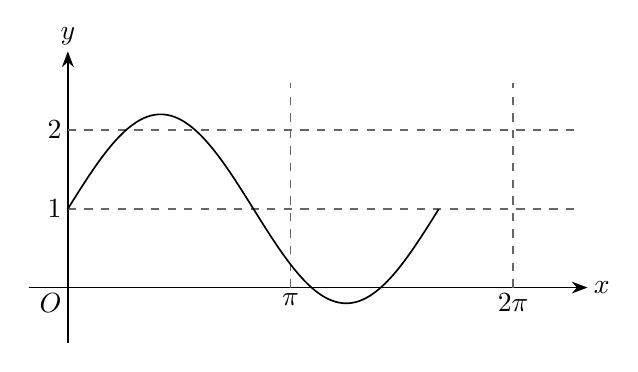
\begin{tikzpicture}[x=1cm,y=1cm,line width=.6pt,>=Stealth,font=\normalsize]
\tikzset{guide/.style={dashed,black!60}}
\draw[->] (-0.5,0)--(6.6,0) node[right,inner sep=0pt,xshift=2pt] {$x$};
\draw[->] (0,-0.7)--(0,3.0) node[above,inner sep=0pt,yshift=2pt] {$y$};
\node[below left,inner sep=0pt,xshift=-2pt,yshift=-2pt] at (0,0) {$O$};
\draw[guide] (0,1)--(6.5,1);
\draw[guide] (0,2)--(6.5,2);
\draw[guide] (2.8274,0)--(2.8274,2.6);
\draw[guide] (5.6549,0)--(5.6549,2.6);
\node[left,inner sep=0pt,xshift=-2pt] at (0,1.0) {$1$};
\node[left,inner sep=0pt,xshift=-2pt] at (0,2.0) {$2$};
\node[below,inner sep=0pt,yshift=-2pt] at (2.8274,0) {$\pi$};
\node[below,inner sep=0pt,yshift=-2pt] at (5.6549,0) {$2\pi$};
\draw[domain=0:4.71,samples=200] plot (\x,{1+1.2*sin(deg(1.2*\x/0.9))});
\end{tikzpicture}
